
%----------------------------------------------------------------------------------------
%	PACKAGES AND OTHER DOCUMENT CONFIGURATIONS
%----------------------------------------------------------------------------------------

\documentclass[12pt]{article} % Default font size is 12pt, it can be changed here
\usepackage{hyperref}
\usepackage{amsmath}
\usepackage{multicol}
\usepackage{geometry} % Required to change the page size to A4
\geometry{a4paper} % Set the page size to be A4 as opposed to the default US Letter
\usepackage{graphicx} % Required for including pictures
\usepackage{float} % Allows putting an [H] in \begin{figure} to specify the exact location of the figure
\usepackage{wrapfig} % Allows in-line images such as the example fish picture

\usepackage{lipsum} % Used for inserting dummy 'Lorem ipsum' text into the template

\linespread{1.2} % Line spacing

%\setlength\parindent{0pt} % Uncomment to remove all indentation from paragraphs

\graphicspath{{./Pictures/}} % Specifies the directory where pictures are stored
\begin{document}

%----------------------------------------------------------------------------------------
%	TITLE PAGE
%----------------------------------------------------------------------------------------

\begin{titlepage}

\newcommand{\HRule}{\rule{\linewidth}{0.5mm}} % Defines a new command for the horizontal lines,
%change thickness here
\center % Center everything on the page

\includegraphics[width=\textwidth]{Glasgow}\\[1.5cm]
\textsc{\LARGE Mobile Human Computer Interaction 4}\\[0.5cm] % Major heading such as course name
\textsc{\Large Assessed Exercise}\\[0.5cm] % Minor heading such as course title

\HRule \\[0.4cm]
{ \huge \bfseries Student Reminder System}\\[0.4cm] % Title of your document
\HRule \\[1.5cm]

\begin{minipage}{0.4\textwidth}
\begin{flushleft} \large
\emph{Author:}\\
Garry \textsc{Sharp}\\
0801585s\\ % Your name
\end{flushleft}
\end{minipage}
~
\begin{minipage}{0.4\textwidth}
\begin{flushright} \large
\emph{Supervisors:} \\
Dr. R. \textsc{Murray-Smith}\\ % Supervisor's Name
\end{flushright}
\end{minipage}\\[4cm]

{\large \today}\\[3cm] % Date, change the \today to a set date if you want to be precise

\vfill % Fill the rest of the page with whitespace

\end{titlepage}

\newpage
\tableofcontents
\newpage

\section{Research and Review}
\subsection{Gathering User Requirements}

\subsubsection{Background}
As the term "reminder system" is applicable to many different configurations and interpretations as to what exactly a reminder system may entail, exercising a good amount of research into gathering realistic user requirements is paramount to the successful completion of this task. Firstly, as the system is geared towards students, the type of reminder should be applicable to a typical student's life, for instance, academic deadlines should be a feature as well as non-academic reminders (perhaps things related to student income management or exercise schedules). Furthermore the system should be versatile enough to be useful to not just an archetypal university students, but also to different caliber's of students, encapsulating part-time and full-time studies as well as the level of the course.
\subsubsection{Requirements Capture}
The requirements capture was geared towards analysing what a vast array of students, from different backgrounds, would like to see in a system. As this type of analysis is dependant upon reaching a broad audience, some form of digital questionnaire system would seem approapriate to this task. This is exactly what was done in order to glean user requirements. A surveymonkey was distributed to via facebook and friends of friends were encouraged to participate, allowing students from universities all over the United Kingdom to present their opinions. The questions allowed for certain tasks to be given a priority which then corresponded to the amount of time and resources that would be invested in that task (which was necessary given the task).

\subsection{Results}

The results showed that out of 20 people who responded to the survey, 17 made the inclusion of a goal driven service as well as a reminder based service as their first and second choices. Examining the reminder based service, location based 

\centerline{
\begin{tabular}{ l l l l l l l l l l l l l l l l l l l l l  l }
Task \& Score &\multicolumn{20}{l}{Participant's Rankings}&Avg\\
\hline
Reminders&2&1&1&1&1&1&2&2&2&2&1&1&2&3&3&3&2&1&2&1&1.7\\
Goals&1&2&2&2&2&2&1&1&1&1&2&2&1&1&2&2&1&2&1&2&1.55\\
History&3&4&5&3&4&5&3&4&5&3&4&3&3&4&5&1&4&5&3&4&3.75\\
Time Tracker&4&5&3&4&5&4&4&5&4&4&5&5&4&5&1&4&5&3&4&5&4.15\\
Social Tracker&5&3&4&5&3&3&5&3&3&5&3&4&5&2&4&5&3&4&5&3&3.85\\
\end{tabular}
}

\subsection{Similar Systems}

\subsubsection{COL Reminder}
COL Reminder is an android based app (available on the app market) that is a time based reminder service. You are able to add a number of timed reminders that fire when the android clock time is equal to the time set in the reminder. the app has a straightforward interface and is reasonably simple to use. 
\subsubsection{Spoty Lite Location Reminder}
Spoty Lite is a location based reminder service that gives the user the ability to fire a reminder event when the user is at a certain location. This app also encouraged me to use the Fake Location app that allows people to simulated a GPS location. This proved to be extremely useful in both testing and demonstrating the app that I built.

subsection{Sample Scenarios}
\begin{description}
\item[Scenario 1] \hfil\\
A user wants to set a goal for number of hours spent studying Mobile HCI. They go into the app's goals' activity and add a goal. Later as they accomplish milestones in achieving the goal, they are able to update the app, increasing their overall progress. Eventually all milestones are accomplished and the goal is removed from the system.
\item[Scenario 2] \hfil\\
A user want's to dedicate 1 hour to studying before leaving to go to the library to return a book. They set the alarm and after an hour they are reminded to go to the library and return the book. The user does not have to worry about removing this reminder from the system as this is all done automatically.
\item[Scenario 3] \hfil\\
A user wishes to be reminded that they have to return an overdue book next time they are close to the library. They set a location based alarm which is triggered when the user is within 50 meters of the location.
\end{description}

\section{Design}
\subsection{Core Functionality}
The dichotomy between the reminders/goals and the other proposed functionality is extensive, as such, the two primary features of the app are goals and reminders. Additional features will only be added if time permits. A Full list of requirements includes.

\begin{description}
\item[Reminders] \hfil\\
A system that allows users to set reminders and fires them when approapriate.
\item[Goals] \hfil\\
A system that allows users to add goals, complete them, remove them, and show an overall progress.
\item[Persistent Storage] \hfil\\
Items should exist beyond the apps lifecycle. For this reason a custom database should be created.
\item[Run in Background] \hfil\\
Reminders should be able to run in the background and fire even if no activities are currently running.
\end{description}

\subsection{Implementation Discussion}

One of the requirements for the system was that it had to be written for an android device. This meant that there was a choice bwteen using the native android SDK or using the Phonegap/Cordova plugin and writing the project using a HTML, CSS and Javascript/jQuery combination. My decision to use native android was born of a knowledge of the two systems. Having previously used both Phonegap and native android, I hold the opinion that phonegap is very good for short projects, wheras the strength and versatility of the native android platform often suits larger scale projects more aptly. Further to this, I believe that phonegap excels when trying to make applications that would act and appear similar to how a mobile website would appear. 

\subsection{Designing the User Interface}

\subsubsection{Goals}

\begin{wrapfigure}{r}{0.47\textwidth}
\begin{center}
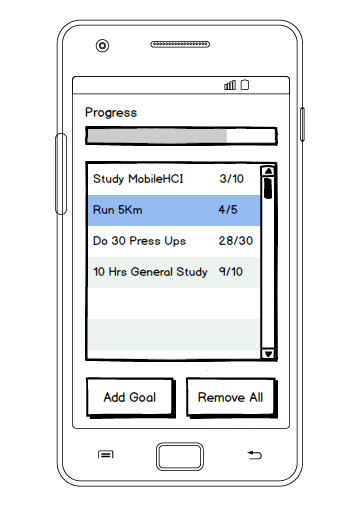
\includegraphics[width=0.47\textwidth]{Goals}
\caption{goal Activity Wireframe}
\end{center}
\end{wrapfigure}

The goal system allows users to add goals and then remove these golas by either selecting remove all or by completing the goals. Due to the variety of how a goal can be completed, it is quite difficult to build a system that can accurately detect when a goal's milestone has been completed or when a goal has been accomplished. For instance, if using location, it would be difficult to distinguish between when a user has simply walked past the library and when the user has actually visited the library. For this reason, milestones in goals are incremented when the user clicks on the item, incrementing the value. Additionally all goals take a format of a description, type (which isn't actually used in this version of the program) and an upper and lower limit. When the lower value has been incremented enough times and matches the target/upper value. The goal is removed as it has been completed.


\subsubsection{Reminders}

As there are two reminder features (one location based, the other time based). It seemed non-sensical to make the user navigate through a series of menus and so tabs were decided on from a very early phase of the user interface design. Looking specifically at the location based reminder, there are two schools of thought for analysing the mechanism that is used to get the desired alert locations. This is manual input vs list selection. Interestingly both of these options subscribe to the well known HCI problem of deciding when to use a command-line iterface and when to use a menu-driven interface. In normal systems, a menu-driven interface can be slower for an expert user but more efficient for novice and intermediate users. In the system that I have designed, the user is prompted to select from one of four pre-programmed locations where the reminder can be triggered. Manually enterring the location was finally not implemented as the menu driven interface provides a both faster, and more convenient user experience.

\begin{figure}[H]
\begin{minipage}[h]{0.45\linewidth}
\centering
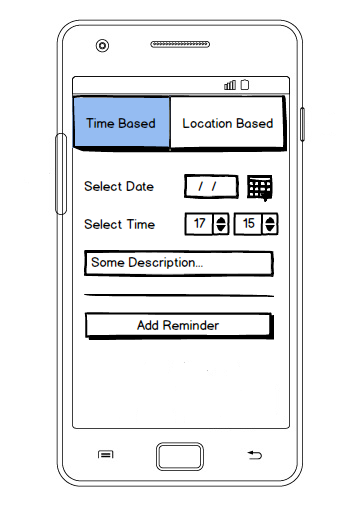
\includegraphics[width=\textwidth]{Reminder1}
\caption{Time Based Reminder}
\label{fig:figure1}
\end{minipage}
\hspace{0.5cm}
\begin{minipage}[h]{0.45\linewidth}
\centering
\includegraphics[width=\textwidth]{Reminder2}
\caption{Location Based Reminder}
\label{fig:figure2}
\end{minipage}
\end{figure}


\section{Evaluation}
\subsection{Acceptence Testing}

The program works correctly and has not crashed in its current state. Acceptence testing, due to time restrictions, meant that features were tested locally after implemention. No formal test suite has been applied, nor has any other form of black box testing. More robust testing strategies are described in the Further Work section of this report later on.
\subsection{User Testing}

It should be noted that the user evaluation focussed on the usability of the system rather than if the system met the requirements gleaned from the initial requirements questionnaire. A number of testing stategies were considered, but finally task-oriented hall intercept testing was chosen. Hall intercept testing is based on Jakob Neilson's claim that "5 users is enough", which in turn is based on the mathematical model which states the proportion of discovered problems U. \[ U = 1 - (1 - p)^n  \] where p is the probability of any one individual finding an error and n is the number of participants. It's main principle is that participants, if willing, should be random members of the public (people you would intercept in the hall), as this naturally selects a cross section of society relevant to the app and also removes user bias as they have no vested interest in either the app, its development or the experiment.

Users were asked to complete a series of tasks and comment on anything that they found difficult. User's were also left with the app until an event fired (a timed reminder) and were also asked to comment on this.  The response received was very positive and many said that if the app were launched commercially (together with more advanced features) that they would consider using it. When a few used were asked the impromptu question of whether they would or would not pay for the app, all reponded that they would not. Inferring that the app would perhaps work well with advertisements being its primary revenue stream if released commercially.

\section{Shortcomings}

There are a number of aspects of the system that could function better. Firstly, unlike other location based apps (such as Spoty), there is no distinction between large areas and small areas. For instance, being 50 meters from the center of the Glasgow University Library means that actually a user must be quite close to the outside of the building before the event is triggered. 50 meters was chosen arbitrarily and a good improvement of this would allow the user to specify the distance away from the target before they set the reminder.

Another improvement that could be made is that the app could be made much more customisable with history and settings views added.


\section{Further Work}

There are many avenues that can be explored when thinking about how the app could be expanded in the future, this list is extensive and so a full list of desired functionality is omitted, however some examples might include: 

\begin{itemize}
\item Ability to add custom locations to the location list.
\item More operations for goal items, especially ones that are specific to its type.
\item More customisable alerts (beeps or vibrate enabled/disabled).
\item Sharing reminders with people.
\item More intelligent reminders that fire in more specific circumstances (for instance if someone has been at the library for at least 5 mins)
\end{itemize}

The user experience would, invariably, be vastly improved by the addition of some of these features. It is important to realise that the time available for the creation of this project was constrained in the sense that there are many other demands on time for other academic pursuits. In this regard, a vastly greater system could be realised with greater time investment.

Natural consequences of this would involve a much more robust and less error prone system. This is due to the added time and resources that would be available for user testing. I imagine that testing wouldn't take a much different approach concerning the usability (with perhaps a few more participants and more tasks in the interest of being thourough). Where testing differs is in the consideration of how the app meets people's needs, if it conforms to a requirements set and also if additional requirements must be considered as a result of this testing. For this I believe the best approach for would be to run a test suite, combined with redeploying the initial requirements questionnaire alongside the app to see if it meets users needs.

Content
Test
Risk

\section{Refs}

Virzi, R.A., Refining the Test Phase of Usability Evaluation: How Many Subjects is Enough? Human Factors, 1992. 34(4): p. 457-468. 








\end{document}